\externaldocument{../appendix/chapter_app}
\externaldocument{../4/chapter_algorithm}
\externaldocument{../3/chapter_modeling}
\startchapter{Evaluation}
\label{chapter:Exp}
This evaluation aimed to experimentally evaluate the model for communication analysis and the identification algorithms. It focus on evaluating the model and and algorithms. By the evaluation, it should be able to know if the captured dual\_traces contain sufficient information of the communication model in ChapterChapter\ref{chapter:Mod}. The evaluation also verify the design of the algorithms, for their correctness and efficiency.  

User case study is not included in this thesis and can be the future work. The feature prototype implementation is not evaluated and can be part of the user case study. But I used the implemented feature on Atlantis to conduct the evaluation experiments.

In this section, I describe the design of the evaluation. Two Evaluation experiments are conducted for this evaluation.  All the programs in these two experiments were written in C++ and the source code can be found in Section\ref{expcode}. Our search partner DRDC provided the captured traces, the used .dll files and  the source code of the programs for the experiments. Evaluation results are provided for each experiment. At the end, I discuss the result of the experiments.  

\section{Evaluation Experiments}
Both of the conducted experiments are about named pipe communication method. The following two subsections provides the details of the experiments and their result.
\subsection{Experiment 1}
In the first experiment, two programs communicated with each other through a synchronous Named pipe channel. One of the programs acted as the Named pipe server while the other as the client. Figure\ref{exp1} is the sequence diagram of the interaction between the server and client. Traces were captured while these two program were running and interacting. The two captured traces are analysis as dual\_trace $exp1$ in this experiment. I used the implemented features in Atlantis to analyse this dual\_trace. I ran the ``Stream identification" and ``Communication identification" operations for this dual\_trace. The identified streams, communication and the processing time are listed in Table\ref{resutl1}.

\begin{figure}[H]
\centerline{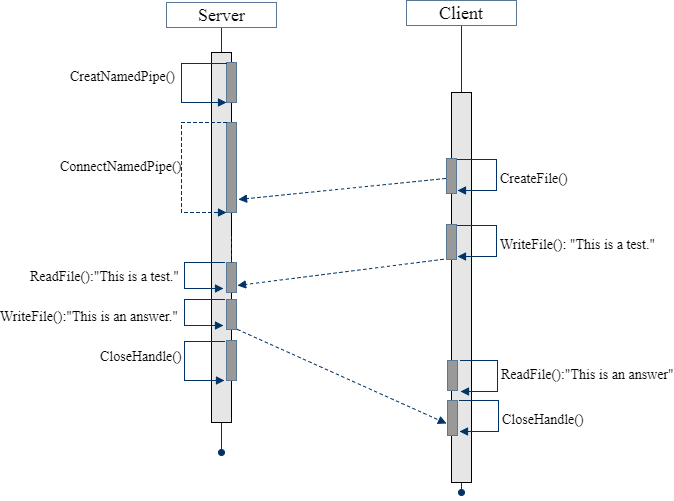
\includegraphics[scale=0.7]{Figures/exp1}}
 \caption{Sequence Diagram of Experiment 1}
\label{exp1}
\end{figure}

    \begin{table}[H]
        \centering
        \caption{Dual\_trace  $exp1$  Analysis Result}
        \label{result1}
        \begin{tabular}{|l|l|l|l|}
            \hline
             \multirow{2}{*}{\textbf{}} &
               \multicolumn{2}{c|}{\textbf{Stream Identification}} &
                \multirow{2}{*}{\textbf{Communication Identification}}\\
             \cline{2-3}
              &Server &Client &   \\
              \hline
              \textbf{Result} & & &   \\
             \hline
               \textbf{Processing Time}& \multicolumn{2}{c|}{}&  \\
              \hline
        \end{tabular}
    \end{table}

\subsection{Experiment 2}
In the second experiment, one program was running as the Named pipe server, while four other programs as the Named pipe clients connected to this server. Those four clients (client 1, client 2, client 3 and client 4) used the identical program but run in sequence. Figure\ref{exp2} is the sequence diagram of  the interaction among the server and clients. Traces were captured at the time when these five programs were running and interacting. One trace for each program. I only analyzed  three traces which are considered as two dual\_traces, $exp2.1$ and $exp2.2$. $exp2.1$ consist of traces of server and client 1 and $exp2.2$ consist of traces of server and client 2. I also ran the ``Stream identification" and ``Communication identification" operations for these two dual\_trace. The identified streams, communication and the processing time are listed in Table\ref{resutl21} and Table\ref{resutl21}


    \begin{table}[H]
        \centering
        \caption{Dual\_trace  $exp2.1$  Analysis Result}
        \label{result21}
        \begin{tabular}{|l|l|l|l|}
            \hline
             \multirow{2}{*}{\textbf{}} &
               \multicolumn{2}{c|}{\textbf{Stream Identification}} &
                \multirow{2}{*}{\textbf{Communication Identification}}\\
             \cline{2-3}
              &Server &Client &   \\
              \hline
              \textbf{Result} & & &   \\
             \hline
               \textbf{Processing Time}& \multicolumn{2}{c|}{}&  \\
              \hline
        \end{tabular}
    \end{table}

    \begin{table}[H]
        \centering
        \caption{Dual\_trace  $exp2.2$  Analysis Result}
        \label{result22}
        \begin{tabular}{|l|l|l|l|}
            \hline
             \multirow{2}{*}{\textbf{}} &
               \multicolumn{2}{c|}{\textbf{Stream Identification}} &
                \multirow{2}{*}{\textbf{Communication Identification}}\\
             \cline{2-3}
              &Server &Client &   \\
              \hline
              \textbf{Result} & & &   \\
             \hline
               \textbf{Processing Time}& \multicolumn{2}{c|}{}&  \\
              \hline
        \end{tabular}
    \end{table}



\begin{figure}[H]
\centerline{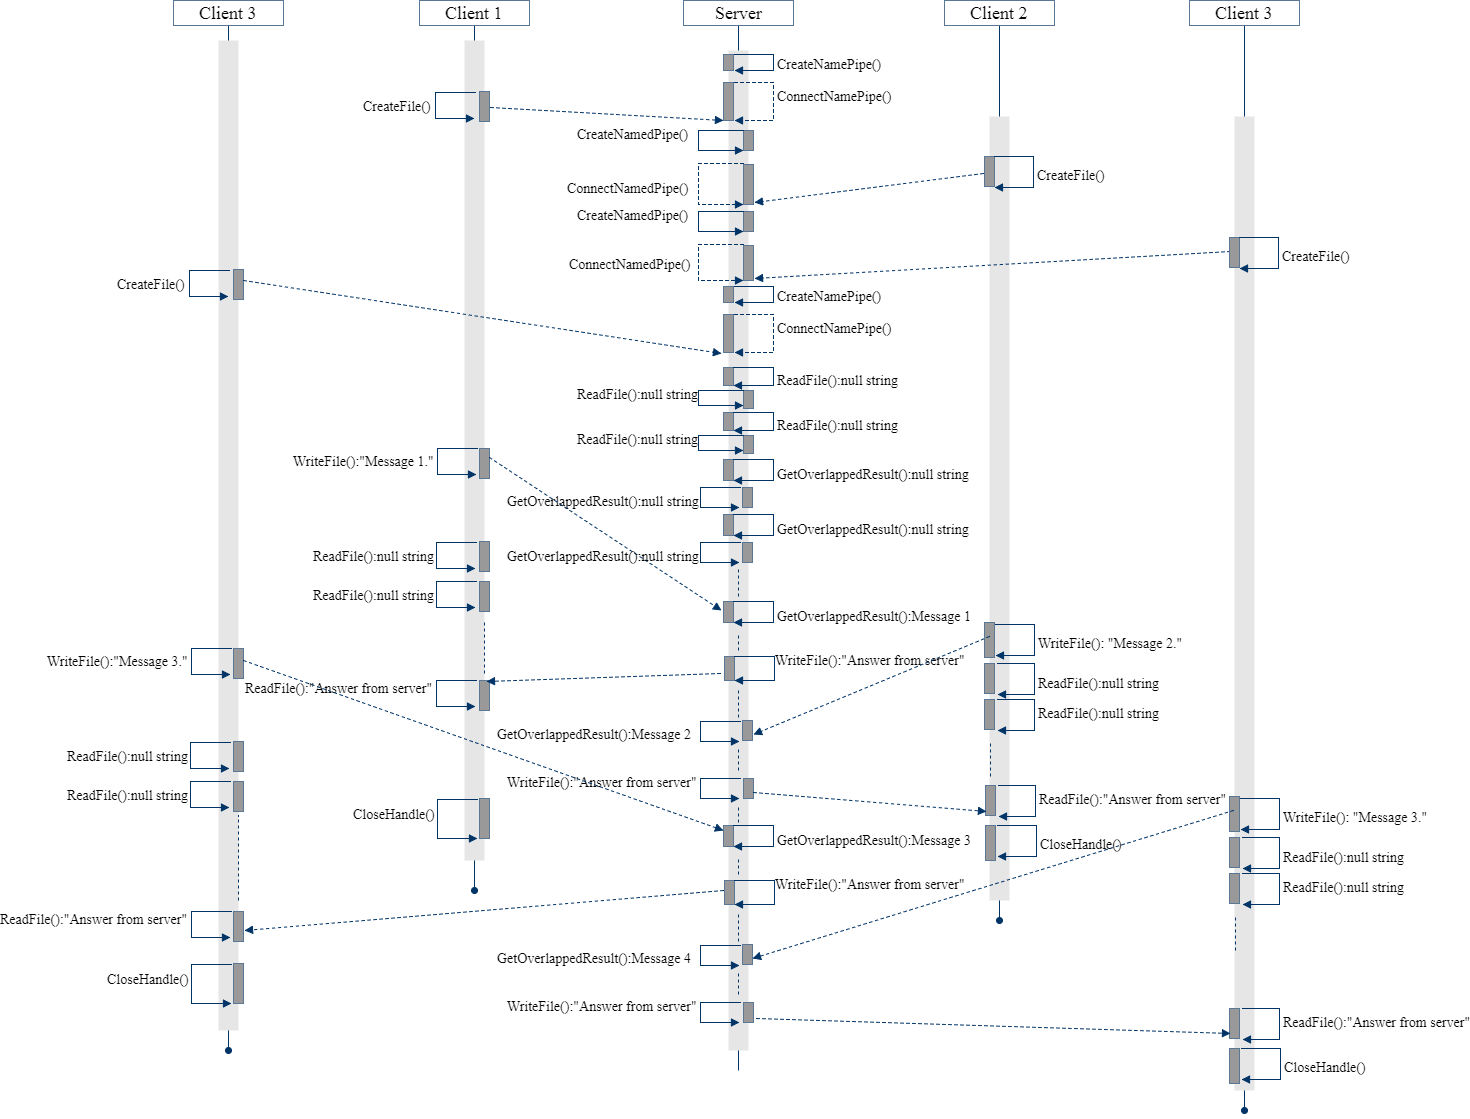
\includegraphics[scale=0.4]{Figures/exp2}}
 \caption{Sequence Diagram of Experiment 2}
\label{exp2}
\end{figure}

\section{Discussion}
The identification result and the processing time of the identifications of each experiment are listed in Table\ref{expresult}. All communications in the dual\_traces are being successfully identified. However, dual to the channel id and transmitted data of the communication between server and client 1 was identical to those of the communication  between server and client 2. There is one false negative error in exp2.1 and one in exp2.2 which is align to the explanation in Section\ref{streammatch}. The dual\_traces being analysed is relatively small, so that the processing times of the identification are acceptable. Fortunately, according to the time complexity of the main algorithm of the identification which is O(N+M), the processing time will only grow linearly corresponding to the size of the dual\_trace.

   




